\chapter{Implementação}

O conjunto de sistemas embarcados propostos são integrados em um Controlador Semafórico, dispondo um meio de monitorar, controlar e gerenciar os vários aspectos envolvidos no ambiente urbano, em relação ao trânsito. O controlador semafórico é uma solução que envolve diferentes equipamentos, com objetivos específicos cada, que interligados apresentam um meio de ordenar o fluxo veicular e de pedestres em seu entorno.

Com a utilização de microcontroladores, o planejamento de circuitos eletrônicos e a programação de firmwares dedicados, o controlador semafórico é responsável por realizar o acendimento e monitoramento da sinalização semafórica, sendo suas funções mais relevantes para tal solução: acendimento de grupos focais (lâmpadas de semáforos) veiculares, acendimento de grupos focais para pedestres, detecção de demanda de travessia de pedestres, sinalização de tempo restante de passagem de veículos (display acoplado aos grupos focais, exibindo um contador regressivo).

Cada sistema, individualmente, possui um propósito específico, e foi planejado de modo otimizado, para apresentar confiabilidade, fácil funcionamento e custo reduzido. Os microcontroladores utilizados para alcançar os objetivos foram da família PIC e da família AVR, sendo, especificamente, o PIC16F77, PIC12F675 e AT89S8253. Em cada aplicação, diferentes funcionalidades dos microcontroladores foram utilizadas, dependendo das necessidades apresentadas.


\section{Placa de controle de acendimento semafórico}

\begin{figure}[ht]
    \begin{center}
    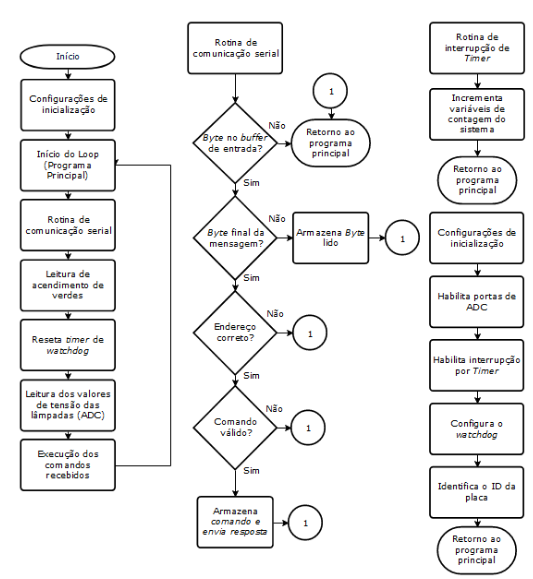
\includegraphics[width=0.8\textwidth]{figuras/fluxo_fase.PNG}
    \end{center}
    \caption[Placa de fase]{Fluxograma de funcionamento do firmware da placa de controle de acendimento.}
    \label{placa_fase}
\end{figure}

A placa de controle de acendimento semafórico tem como função assegurar o funcionamento correto do semáforo, tanto veicular quanto de pedestres, sendo responsável pelo acendimento e monitoramento dos focos, assegurando a sequência correta de cores do semáforo (Verde > Amarelo > Vermelho).
%[http://meusite.mackenzie.br/professor_cucci/ManualSemaforos2014.pdf]. 

O microcontrolador utilizado na placa é um PIC16F77, que possui 40 pinos e capacidade de processamento de 8 bits. Um cristal é utilizado, para gerar uma velocidade de clock de 20 MHz, e cada instrução é realizada a cada 200 ns (4 ciclos do clock). Esse dispositivo é utilizado para chavear a tensão da rede elétrica e monitorar o acendimento semafórico, e enviar as informações para a central do controlador semafórico.

O firmware da placa foi escrito especificamente para o dispositivo utilizado realizar as funções desejadas. A Figura \ref{placa_fase} apresenta os processos realizados pelo microcontrolador durante o seu funcionamento. A placa aguarda os comandos vindos da central (CPU) do controlador semafórico para executar o acendimento dos focos. Os comandos são recebidos pela porta serial (USART) do PIC16F77, através de comunicação assíncrona.

O acendimento de cada foco é realizado com a utilização de um optoacoplador, em conjunto com um TRIAC. O optoacoplador é um dispositivo que permite o isolamento de dois circuitos, utilizando luz emitida por um LED para acionar a outra parte do circuito, 
%[Rudolf F. Graf (1999). Modern dictionary of electronics. Newnes. ISBN 0-7506-9866-7.], 
enquanto o TRIAC é um dispositivo que permite a passagem de corrente nas duas direções, a partir de ativação através de um terceiro pino. 
%[M.D. Singh, K.B. Khanchandani, Power Electronics, Second Edition, Tata McGraw-Hill, New Delhi, 2007, pages 148-152]. 
Utilizando esses dois componentes, é possível realizar o controle da tensão da rede elétrica (220 V) utilizando um sinal de 5 V dos pinos de I/O do microcontrolador.

O acendimento de cada foco é dado pelo controle do pino do PIC responsável por cada cor (verde, amarelo, vermelho). Ao executar o comando de acender foco, o pino é colocado em 0 V, ativando assim o optoacoplador, e fazendo passar o neutro, da rede elétrica, para o foco semafórico, resultando em seu acendimento.

\begin{figure}[ht]
    \begin{center}
    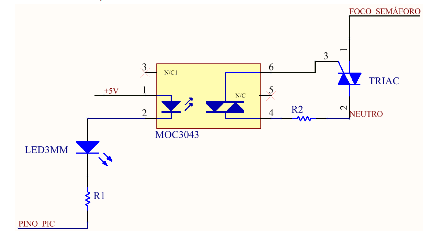
\includegraphics{figuras/moc_triac.PNG}
    \end{center}
    \caption[Acendimento semafórico]{Circuito responsável pelo acendimento semafórico.}
    \label{moc_triac}
\end{figure}

O PIC16F77 possui um conversor A/D com precisão de 8 bits, que é utilizado, no projeto, para realizar a leitura do valor da tensão da carga, que é o foco, quando aceso. O sinal passa por um transformador abaixador e uma ponte retificadora, para ser lido pelo pino do PIC, que resulta em um valor de leitura proporcional à potência da carga utilizada. Esse circuito permite ao sistema ter capacidade de monitorar diversos estados das lâmpadas utilizadas no semáforo, sendo eles subtensão, funcionamento esperado, sobretensão e queima.

\begin{figure}[ht]
    \begin{center}
    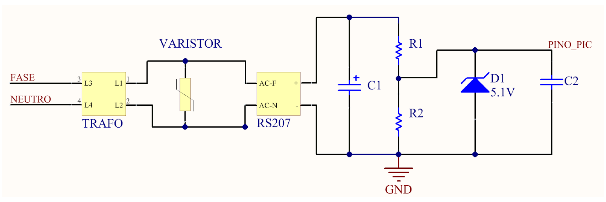
\includegraphics[width=0.5\textwidth]{figuras/trafo.PNG}
    \end{center}
    \caption[Detecção da lâmpada]{Circuito responsável pela leitura do sinal analógico.}
    \label{trafo}
\end{figure}

Outra função da placa é o monitoramento de acendimento dos focos, em que o PIC realiza a leitura de cada foco (verde, amarelo, vermelho) de uma fase e armazena os valores lidos. A leitura é realizada no pino de saída de um optoacoplador, o qual é ativado pela presença de fase e neutro (rede elétrica) na sua entrada. A placa possui um circuito separado para cada foco monitorado, cada um ocupando um pino diferente de I/O do PIC.

\begin{figure}[ht]
    \begin{center}
    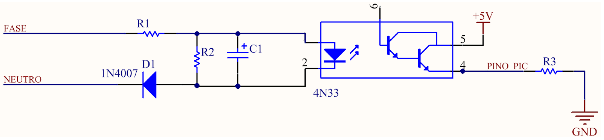
\includegraphics[width=0.5\textwidth]{figuras/4n33.PNG}
    \end{center}
    \caption[Detecção de presença de fase]{Circuito responsável pelo monitoramento de acendimento dos focos.}
    \label{4n33}
\end{figure}

Além das funções já mencionadas, o PIC é configurado para habilitar interrupção por timer. O timer é utilizado como contador para o controle das funções temporizadas do sistema. 

\section{Placa de controle de contagem de tempo semafórico}

\begin{figure}[ht]
    \begin{center}
    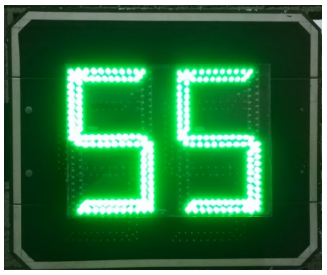
\includegraphics{figuras/cronometro.PNG}
    \end{center}
    \caption[Sistema de cronômetro]{Cronômetro marcador de tempo semafórico.}
    \label{cronometro}
\end{figure}

A placa de controle de contagem de tempo semafórico tem como finalidade realizar a contagem, e mostrar no display, como mostrado na Figura \ref{cronometro}, do tempo de passagem veicular, enquanto o grupo focal estiver aceso no estado verde.

O microcontrolador utilizado é um AVR AT89S8253, que possui 40 pinos e capacidade de processamento de 8 bits. Um cristal é utilizado, para gerar um clock de 12 MHz, e cada instrução é realizada a cada 12 ciclos do clock. O dispositivo é utilizado para realizar as funções de detectar o acendimento do verde no semáforo, contar, e salvar em memória, o tempo de verde e exibir o tempo em um display de 7 segmentos. O fluxo do firmware utilizado nesse microcontrolador pode ser visualizado na Figura \ref{fluxo_cron}.

\begin{figure}[ht]
    \begin{center}
    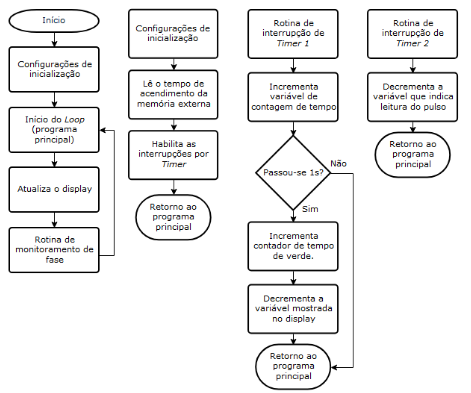
\includegraphics{figuras/fluxo_cron.PNG}
    \end{center}
    \caption[Fluxograma do sistema de cronômetro]{Funcionamento do firmware do sistema de contagem de tempo semafórico.}
    \label{fluxo_cron}
\end{figure}

O equipamento de contagem é instalado acoplado ao foco semafórico e é eletricamente conectado em paralelo com a fase verde do semáforo. Como não existe comunicação entre a placa de cronômetro e o controlador semafórico, o início da contagem do tempo é determinado pela detecção de acendimento do semáforo. Ao detectar a presença da rede elétrica, o microcontrolador busca na memória o valor da contagem de tempo de verde e inicia a contagem regressiva. Caso não exista valor salvo na memória, é carregado um valor padrão.

\begin{figure}[ht]
    \begin{center}
    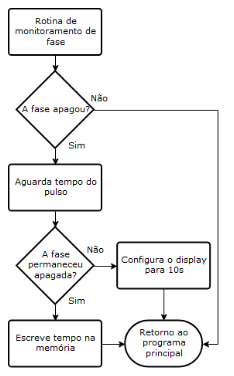
\includegraphics{figuras/fluxo_cron2.PNG}
    \end{center}
    \caption[Fluxograma do monitoramento do cronômetro]{Fluxo da rotina de monitoramento da fase veicular.}
    \label{fluxo_cron2}
\end{figure}

Após iniciar a contagem, o microcontrolador passa a monitorar a fase acesa, de acordo com a rotina demonstrada na Figura \ref{fluxo_cron2}. O controlador semafórico possui um método para indicar que o tempo de verde está próximo do fim, na forma de um pulso, com duração de 100 ms, durante o qual a alimentação é retirada da placa de contagem. Esse método é importante para assegurar o funcionamento correto do sistema nas determinadas situações:

\begin{itemize}
\item No ciclo inicial, em que o microcontrolador ainda não possui valor de tempo gravado na memória.
\item Após mudanças dos planos, quando o tempo de acendimento passar a ser diferente do tempo armazenado na memória.
\end{itemize}

O pulso é necessário nessas situações, pois são cenários em que ocorre dessincronização entre a placa de contagem e o controlador semafórico, e os displays não exibem o tempo correto. Ao reconhecer o pulso, porém, a placa entra em sincronia com o controlador e exibe o valor correto no mostrador (o pulso indica que faltam 10 s de tempo de verde). Ao apagar o foco verde, o microcontrolador reconhece a ausência de alimentação por mais de 100 ms, e salva na memória o tempo do ciclo de acendimento.
No equipamento são utilizados dois timers distintos para gerar interrupções. O primeiro é utilizado para a contagem do tempo e atualização da variável que é exibida nos displays. O segundo é utilizado para a contagem dos 100 ms para reconhecimento do pulso do controlador.

\section{Placa de detecção de demanda de atuadores externos}

\begin{figure}[ht]
    \begin{center}
    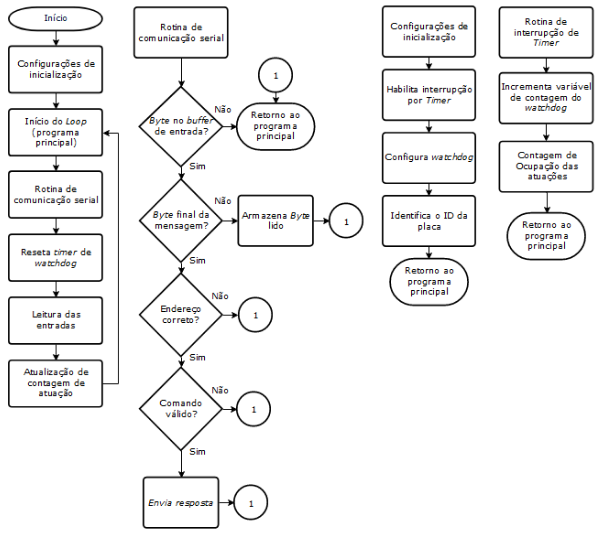
\includegraphics{figuras/fluxo_atdr.PNG}
    \end{center}
    \caption[Fluxograma do atuador]{Fluxo do funcionamento de detecção de demanda.}
    \label{fluxo_atdr}
\end{figure}

A placa de monitoramento de demanda de atuadores externos tem como finalidade acumular as demandas vindas de atuadores externos, ativados por pedestres para realizar a travessia de vias. A placa recebe um sinal, referente às atuações, do equipamento que realiza o registro das demandas, à medida que vão ocorrendo, e utiliza esse sinal para realizar cálculos referentes à quantidade e volume de demandas registradas.

Assim como a placa de controle de acendimento semafórico, o microcontrolador utilizado nessa placa é um PIC16F77, utilizando, também, um cristal de 20 MHz para gerar o clock. As funções necessárias para essa placa são:

\begin{itemize}
\item Comunicação com a CPU
\item Registro de atividades de atuadores externos
\item Cálculo de quantidade de demanda em um determinado intervalo de tempo
\item Cálculo de volume de demandas em um determinado intervalo de tempo
\end{itemize}

O firmware escrito para essa placa segue o fluxo que pode ser visto na Figura \ref{fluxo_atdr}, que apresenta os processos realizados pelo microcontrolador durante seu funcionamento. Para realizar a comunicação com a CPU, é utilizada a porta serial do PIC, através de uma comunicação assíncrona. 

\begin{figure}[ht]
    \begin{center}
    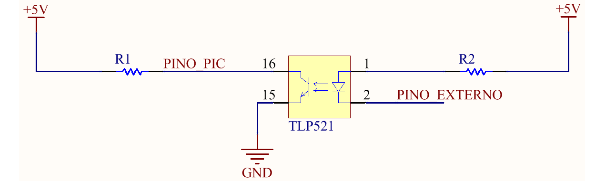
\includegraphics{figuras/atuacao.PNG}
    \end{center}
    \caption[Circuito de atuador]{Circuito responsável pela detecção de atuação.}
    \label{atdr}
\end{figure}

Como pode ser visto na Figura \ref{atdr}, o circuito de monitoramento das demandas possui um optoacoplador, que é ativado quando o equipamento que registra as demandas envia o sinal por meio do pino externo, e o PIC detecta a atuação. Além desses dados, o PIC incrementa uma contagem cada vez que uma demanda é registrada, desse modo armazenando a contagem de atuação para cada detector.

Além da contagem de atuação, outra funcionalidade da placa é o armazenamento do volume das atuações. Para isso, o timer do microcontrolador é utilizado. Durante a rotina de interrupção do timer, o PIC identifica as demandas recebidas e calcula, durante uma janela de tempo (determinada pela CPU), durante que porcentagem desse período as demandas ficaram ativas. Essas informações armazenadas são enviadas para a CPU, por meio da porta serial, quando requisitadas.

\section{Placa de registro de demanda de pedestre}

A placa de registro de demanda de pedestre é um sistema de botoeira que registra as demandas realizadas pelo pedestre e envia um sinal para o controlador semafórico como aviso de ativação. O equipamento possui um botão, que deve ser pressionado para que ocorra o registro da demanda. 

O microcontrolador utilizado na placa é um PIC12F675, que possui 8 pinos e capacidade de processamento de 8 bits. É utilizado o oscilador interno do PIC, com velocidade de clock de 4 MHz, e cada instrução é realizada a cada 4 ciclos do clock. Esse dispositivo é utilizado para detectar o pressionamento do botão que realiza a requisição de demanda, enviar um sinal ao controlador para identificar o registro, detectar o acendimento da fase de pedestres e ativar o funcionamento de um buzzer para indicar a travessia, no modo sonoro. 

\begin{figure}[ht]
    \begin{center}
    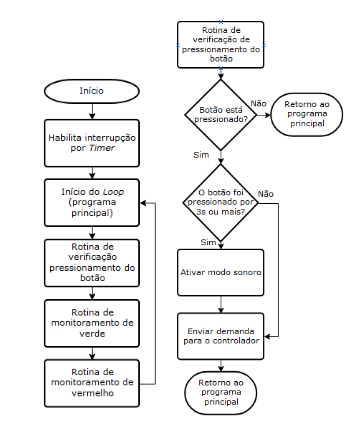
\includegraphics{figuras/fluxo_bot.PNG}
    \end{center}
    \caption[Fluxograma botoeira]{Rotina principal da placa de registro de demanda de pedestre.}
    \label{fluxo_bot}
\end{figure}

O fluxo da rotina principal do firmware utilizado no dispositivo pode ser visto na Figura \ref{fluxo_bot}. O PIC realiza a leitura do botão por meio de polling do pino (leitura do estado do botão a cada ciclo do programa principal). O equipamento possui dois modos de funcionamento, dependendo do pressionamento do botão, sendo eles o modo sonoro, caso o pressionamento ocorra por mais de 3 segundos, e o modo silencioso, no caso de pressionamento por menos de 3 segundos. A reconhecer o pressionamento do botão, a botoeira envia um sinal para o controlador semafórico, para requisitar o acionamento do plano de pedestres. 

Os circuito utilizados, para enviar o sinal de demanda para o controlador, e para ativar o buzzer, são equivalentes, e são representados pelo circuito na Figura \ref{envio_demanda}. Para ocorrer a ativação, um pino do PIC é utilizado para chavear um transistor TBJ, que causa a ativação do relé, fazendo com que o sinal de 12 V seja enviado ao controlador ou ao buzzer. 

\begin{figure}[ht]
    \begin{center}
    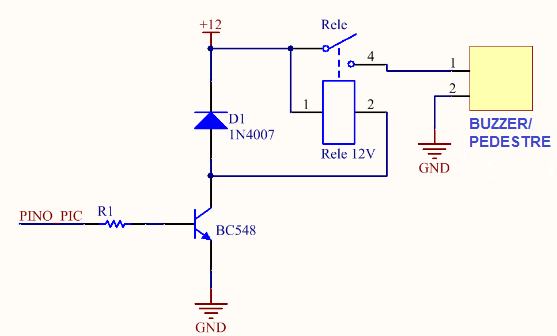
\includegraphics[width=0.7\textwidth]{figuras/envio_demanda.PNG}
    \end{center}
    \caption[Circuito de chaveamento 12V]{Circuito responsável pelo chaveamento da tensão a ser enviada ao controlador ou ao buzzer.}
    \label{envio_demanda}
\end{figure}

Após a leitura do estado do botão e envio do sinal de demanda ao controlador, o equipamento realiza o monitoramento do semáforo de pedestres para determinar em qual estado se encontra.

No caso do modo de funcionamento sonoro, ao detectar o acendimento do foco verde, o equipamento ativa o funcionamento intermitente do buzzer, na frequência de 1 Hz, para indicar ao pedestre que a travessia pode ser iniciada. Esse processo pode ser visto na Figura \ref{verde}. 

Ao detectar que o estado do semáforo passou de verde para vermelho intermitente, o equipamento ativa o funcionamento do buzzer, dessa vez na frequência de 2 Hz, para indicar que o tempo de travessia se aproxima do fim. Ao identificar que o foco vermelho ficou aceso continuamente, o equipamento desliga o buzzer. Esse fluxo pode ser visto na Figura \ref{vermelho}.

Para controlar a frequência de ativação do buzzer, é utilizada a interrupção de timer do microcontrolador. A rotina de interrupção de timer é mostrada na Figura \ref{timer}.

\begin{figure}[ht]
    \begin{center}
    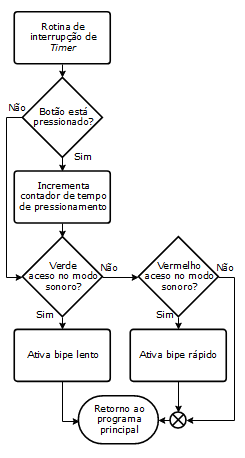
\includegraphics{figuras/rotina_timer.PNG}
    \end{center}
    \caption[Timer da botoeira]{Rotina de interrupção de timer.}
    \label{timer}
\end{figure}

Durante o modo de funcionamento silencioso, a botoeira não realiza nenhuma ação, apenas monitora os acendimentos, sem ativar o buzzer.

\begin{figure}[ht]
    \begin{center}
    \subfloat[]{\label{verde}
    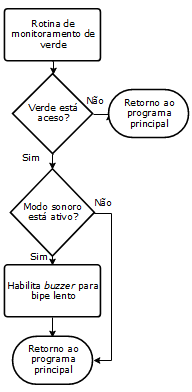
\includegraphics[width=0.4\textwidth]{figuras/monit_verde.PNG}}
    \subfloat[]{\label{vermelho}
    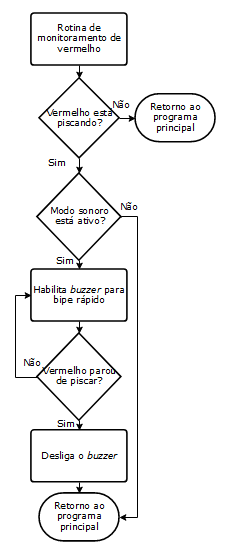
\includegraphics[width=0.4\textwidth]{figuras/monit_vermelho.PNG}}
    \end{center}
    \caption[Fluxos botoeira]{(a)Rotina de monitoramento de acendimento de verde. (b)Rotina de monitoramento de acendimento de vermelho.}
    \label{fluxos}
\end{figure}
